\documentclass[
a4paper,
oneside,
10pt,
fleqn,
headsepline,
toc=listofnumbered, 
bibliography=totocnumbered]{scrartcl}

% deutsche Trennmuster etc.
\usepackage[T1]{fontenc}
\usepackage[utf8]{inputenc}
\usepackage[english, ngerman]{babel} % \selectlanguage{english} if  needed
\usepackage{lmodern} % use modern latin fonts

% Custom commands
\newcommand{\AUTHOR}{Michael Wieland}
\newcommand{\SECONDAUTHOR}{Fabian Hauser}
\newcommand{\INSTITUTE}{Hochschule für Technik Rapperswil}

% Jede Überschrift 1 auf neuer Seite
\let\stdsection\section
\renewcommand\section{\clearpage\stdsection}

% Multiple Authors
\usepackage{authblk}

% Include external pdf
\usepackage{pdfpages}

% Layout / Seitenränder
\usepackage{geometry}

% Inhaltsverzeichnis
\usepackage{makeidx} 
\makeindex

\usepackage{url}
\usepackage[pdfborder={0 0 0}]{hyperref}
\usepackage[all]{hypcap}
\usepackage{hyperxmp} % for license metadata

% Mathematik
\usepackage{amsmath}
\usepackage{amssymb}
\usepackage{amsfonts}
\usepackage{enumitem}

% Images
\usepackage{graphicx}
\graphicspath{{images/}} % default paths

% Boxes
\usepackage{fancybox}

%Tables
\usepackage{tabu}
\usepackage{booktabs} % toprule, midrule, bottomrule
\usepackage{array} % for matrix tables

% Multi Columns
\usepackage{multicol}

% Header and footer
\usepackage{scrlayer-scrpage}
\setkomafont{pagehead}{\normalfont}
\setkomafont{pagefoot}{\normalfont}
\automark*{section}
\clearpairofpagestyles
\ihead{\headmark}
\ohead{\TITLE}
\cfoot{\pagemark}

% Pseudocode
\usepackage{algorithm}
\usepackage{algorithmic}

% Code Listings
\usepackage{listings}
\usepackage{color}
\usepackage{beramono}

\definecolor{DarkPurple}{rgb}{0.4, 0.1, 0.4}
\definecolor{DarkCyan}{rgb}{0.0, 0.5, 0.4}
\definecolor{LightLime}{rgb}{0.3, 0.5, 0.4}
\definecolor{Blue}{rgb}{0.0, 0.0, 1.0}

\lstdefinestyle{eclipse-style}{
	language=Java,  
	columns=flexible,
	showstringspaces=false,     
	basicstyle=\footnotesize\ttfamily, 
	keywordstyle=\bfseries\color{DarkPurple},
	commentstyle=\color{LightLime},
	stringstyle=\color{Blue}, 
	escapeinside={£}{£}, % latex scope within code      
	morekeywords={length},
	numbers=left,
	numberstyle=\tiny\color{black},
	frame=single,
}
\lstset{style=eclipse-style}


% Theorems \begin{mytheo}{title}{label}
\usepackage{tcolorbox}
\tcbuselibrary{theorems}
\newtcbtheorem[number within=section]{definiton}{Definition}%
{fonttitle=\bfseries}{def}
\newtcbtheorem[number within=section]{remember}{Merke}%
{fonttitle=\bfseries}{rem}
\newtcbtheorem[number within=section]{hint}{Hinweis}%
{fonttitle=\bfseries}{hnt}

% Dokumentinformationen
\newcommand{\SUBJECT}{Report}
\newcommand{\TITLE}{Cloud Infrastructre Lab 4}

\begin{document}
	
% Front page
\title{\TITLE}
\subject{\SUBJECT}
\author{\SECONDAUTHOR}
\author{\AUTHOR}
\affil{\INSTITUTE}
\date{\today}
\maketitle

% Table of contents
\tableofcontents


%  03.11.2016, 23:55, as PDF to beat.stettler@ins.hsr.ch. 

% Describe how Qemu KVM and Docker work (technical explanation). Also make sure you highlight the 
% differences, pro’s and con’s. 

% Setup and configuration of the Qemu-KVM environment (with explanations) 

% Qemu network configuration 

% A short manual of how to get the ELK stack up and running in Docker 

% Docker network configuration 

% Docker Compose file for the ELK stack 

% Qemu-KVM and Docker networking configuration files/scripts 

\section*{Einleitung}
Diese Dokumentation erklärt die grundlegenden Funktionen von KVM / QEMU / Libvirt sowie Docker, Docker Composer und Docker Swarm. Es wird gemäss der Aufgabenstellung nicht auf allgemeine Virtualisierungsgundlagen eingegangen. Die Möglichkeit der grafischen Verwaltung (z.B. mit \lstinline|virt-manager|) werden gemäss Besprechung im Praktikum ebenfalls nicht weiter berücksichtigt.
%TODO: Brauchen wir docker swarm?


\section{KVM / QEMU}
\subsection{Grundlegendes}
KVM ist eine Virtualisierungslösung für Linux, die Gebrauch von Virtualisierungstechniken aktueller Prozessorarchitekturen macht. Um KVM nutzen zu können, muss der Prozessor des Hostsystems Hardwarevirtualisierung unterstützen (was bei den meisten neueren Intel und AMD Prozessoren der Fall ist). KVM an sich stellt die direkte Schnittstelle zum Linux-Kernel zur Verfügung, als Virtualisierungsumgebung kommt QEMU zum Einsatz.

\subsubsection{Terminologie}
\begin{description}
	\item[Host System] \hfill \\
	Beherbergt eine Virtualisierungslösung und stellt Funktionen zur Verfügung damit ein Gastsystem laufen kann.
	\item[Guest System] \hfill \\
	Läuft virtuell innerhalb des Host Systems. Befehle werden durch eine Virtualisierungslösung an die Hardware des Hosts weitergeleitet.
\end{description}

\subsubsection{QEMU}
QEMU ist ein Open Source System-Emulator. QEMU kommuniziert direkt via KVM mit dem Kernel und der CPU, um so das Gastsystem möglichst nahe an der Hardware laufen zu lassen. Eine komplette Emulation (Vollvirtualisierung) ist mit QEMU ebenfalls möglich, führt jedoch zu grossen Performanceeinbussen.

\subsubsection{Libvirt}

Libvirt ist eine Umgebung, welche den Betrieb einer virtuellen Umgebung über eine einheitliche API zur Verfügung stellt. Dies für KVM/QEMU aber auch alternative Umgebungen wie XEN.

Unter dem Überbegriff \emph{Libvirt} werden normalerweise folgende Komponenten verstanden:

\begin{description}
	\item[libvirt] \hfill \\
	\lstinline|libvirt| ist die eigentliche Programmbibliothek, welche die funktionen der Virtualisierungslösung abstrahiert.
	\item[libvirtd] \hfill \\
	\lstinline|libvirtd| ist ein Daemon, welcher den Betrieb der virtuellen Umgebung (Maschinen, Netzwerken, Speicherpools etc.) organisiert und verwaltet.
	\item[virsh] \hfill \\
	\lstinline|virsh| ist ein Verwaltungswerkzeug, über welches die \lstinline|libvirt(d)|-Umgebung konfiguriert und kontrolliert werden kann. Mit \lstinline|virsh start VM1| kann z.B. eine virtuelle Maschine gestartet werden.
\end{description}

\subsubsection{Virt-Manager}

Das Programm \lstinline|virt-manager| ist ein grafisches Verwaltungsprogramm, über welches die von Libvirt abstrahierte virtuelle Umgebung gesteuert werden kann. Die Oberfläche wird von RedHat in Python/GTK entwickelt und erinnert z.B. an die klassische Oberfläche von VMWare\textregistered vSphere\texttrademark.

Der Virt-Manager kann sich (wie auch \lstinline|virsh|) über eine Netzwerkverbindung mit einer (headless) Libvirt-Umgebung in Verbindung setzen (d.h., es sind keine grafischen Komponenten auf Serverseite nötig.)

\subsection{Installation}
\subsubsection{Hardwarevirtualisierung vmx/svm}
Damit KVM genutzt werden kann, muss die CPU Hardwarevirtualisierung unterstützen. Dies kann bei neueren Prozessoren im UEFI/BIOS aktiviert werden. Ob die Unterstützung momentan aktiv ist, kann mit folgendem Befehl ermittelt werden\footnote{Achtung: Unter gewissen neue Intel CPUs ist dieser Test aufgrund eines Bugs scheinbar erfolgreich, obwohl die Option noch abgestellt ist. In diesem Fall muss die Option trotzdem noch eingeschaltet werden.}:
\begin{lstlisting}[language=bash]
# Eintrag VMX oder SVM sollten zurueckgegeben werden
egrep '(vmx|svm)' /proc/cpuinfo
\end{lstlisting}


Die nötigen \lstinline|kvm|-Kernelmodule werden unter Fedora bei einem Reboot automatisch geladen. Sollte dies nicht der Fall sein, können sie mit folgendem Befehl geladen werden:
\begin{lstlisting}[language=bash]
lsmod | grep kvm # Sollte kvm ausgeben, falls geladen.

# Ansonsten: Kernel Module manuell laden
sudo modprobe kvm
\end{lstlisting}

Bei selber kompilierten Linux Kerneln kann mit \lstinline|make kvmconfig| die entsprechende Build-Konfiguration aktiviert werden.

\subsubsection{Installation KVM}
Die meisten Linux-Distributionen stellen in den Paket-Repositories KVM, QEMU und Libvirt bereit. Wir verwenden in unseren Beispiel die Linux Distribution \lstinline|Fedora Workstation 24|.

\begin{enumerate}
	\item Installation von KVM, QEMU, Libvirt (von Fedora bereitgestelltes Metapaket)\\ \hfill
		\lstinline|sudo dnf install @virtualization libvirt-docs libguestfs-tools|
	\item Starten des \lstinline|libvirtd|-Dienstes\\ \hfill
		\lstinline|sudo service libvirtd start|
\end{enumerate}

\paragraph{Benutzerzugriff} \hfill \\
Der Benutzer, welcher die Virtuellen Maschinen verwalten soll, muss den Gruppen \lstinline|libvirt| und \lstinline|kvm| hinzugefügt werden (gem. Umgebung von \lstinline|Fedora Workstation 24|)
\begin{lstlisting}[language=bash]
sudo usermod -aG libvirt, kvm $USER
\end{lstlisting}

\subsection{Festplattenimages erstellen}\label{sec:festplattenimages-erstellen}
Festplatten-Images können entweder mit dem Tool \lstinline|qemu-img| erstellt werden, oder alternativ mit Libvirt direkt mit dem Tool \lstinline|virt-install| (siehe nächste Seiten).

In unserem Fall bauen wir aber auf eine bestehendes Festplatten-Image der Mini-Distribution ''CirrOS'' auf.

\subsubsection{Unterstützte Festplattenformate}
QEMU unterstützt als Festplatten Images diverse Formate (die nachfolgende Liste wurde übernommen von \url{https://en.wikibooks.org/wiki/QEMU/Images#Image_types}, Lizenz CC-SA):

\begin{description}
	\item[raw] \hfill \\
	(default) the raw format is a plain binary image of the disc image, and is very portable. On filesystems that support sparse files, images in this format only use the space actually used by the data recorded in them.
	\item[cloop] \hfill \\
	Compressed Loop format, mainly used for reading Knoppix and similar live CD image formats
	\item[cow] \hfill \\
	copy-on-write format, supported for historical reasons only and not available to QEMU on Windows
	\item[qcow] \hfill \\
	the old QEMU copy-on-write format, supported for historical reasons and superseded by qcow2
	\item[qcow2] \hfill \\
	QEMU copy-on-write format with a range of special features, including the ability to take multiple snapshots, smaller images on filesystems that don't support sparse files, optional AES encryption, and optional zlib compression
	\item[vmdk] \hfill \\
	VMware 3 \& 4, or 6 image format, for exchanging images with that product
	\item[vdi] \hfill \\
	VirtualBox 1.1 compatible image format, for exchanging images with VirtualBox.
	\item[vhdx] \hfill \\
	Hyper-V compatible image format, for exchanging images with Hyper-V 2012 or later.
	\item[vpc] \hfill \\
	Hyper-V legacy image format, for exchanging images with Virtual PC / Virtual Server / Hyper-V 2008. 
\end{description}

\subsubsection{Anlegen eines neuen Images ohne \lstinline|virt-install|}
Die Erstellung eines \lstinline|qcow2|-Images Namens \lstinline|test.qcow2| mit einer maximalen Grösse von \lstinline|3GB|. Beim \lstinline|qcow2|-Format wird nicht der ganze Speicherplatz beim erstellen alloziert, sondern erst bei tatsächlicher Belegung\footnote{Damit wird sogenannte ''Überprovisionierung'' möglich, d.h. eine Mehrfachvergabe von tatsächlich verfügbarem Speicherplatz an mehrere VMs. Wichtig: Ist der ''tatsächliche'' Speicherplatz aufgebraucht und das Image hat noch (virtuellen) freien Platz, kann es zu Datenverlust kommen (verursacht durch das Guest-Betriebssystem). Libvirt versetzt zur Vorbeugung in diesem Fall alle VMs in einen standby-Zustand.}.


\begin{lstlisting}[language=bash]
qemu-img create /var/lib/libvirt/images/test.qcow2 3G -f qcow2
virsh pool-refresh default
\end{lstlisting}


\subsubsection{Ablegen eines bestehenden virtuellen Images}

In unserem Beispiel greifen wir auf ein bestehendes Festplatten-Image der Mini-Distribution ''CirrOS'' aus dem OpenStack-Projekt zurück.

Zur Inbetriebnahme laden wir das Image im \lstinline|qcow2|-Format aus dem Internet und speichern es im Ordner \lstinline|/var/lib/libvirt/images/|:

\begin{lstlisting}[language=bash]
sudo wget -O /var/lib/libvirt/images/vm1.qcow2 \
http://download.cirros-cloud.net/0.3.4/cirros-0.3.4-x86_64-disk.img
virsh pool-refresh default
\end{lstlisting}

\subsubsection{Libvirt Storage Pools}

Wir haben beim obenstehenden Hinzufügen von Images jeweils zusätzlich das Kommando \lstinline|virsh pool-refresh default| ausgeführt. Dadurch wird der Libvirt Storage-Pool aktualisiert, damit das neue Image erkannt wird.

Libvirt verwaltet die Speicherorte, von denen virtuelle Images Eingebungen werden können, in sogenannten \emph{Pools}. Ein Pool ist dabei oft ein bestimmter Ordner auf dem Computer oder einem Netzwerklaufwerk, kann aber z.B. auch ein iSCSI Speicher darstellen.

Standardmässig ist unter Fedora der Ordner \lstinline|/var/lib/libvirt/images/| mit dem Namen \lstinline|default| als Pool eingerichtet. Diesen haben wir in unseren Beispielen immer verwendet.

Die Pools können mit \lstinline|virsh| wie folgt verwendet werden (Ausschnitt aus \lstinline|virsh help|):

\lstinputlisting{appendix/kvm/libvirt/pool_virsh.man}

Die XML-Konfiguration des \lstinline|default|-Pools sieht wie folgt aus:

\lstinputlisting[caption=\lstinline|/etc/libvirt/storage/default.xml|,language=xml]{appendix/kvm/libvirt/pool_default.xml}



\subsection{Erstellen der virtuellen Maschinen}


\subsubsection{Virt-Install}\label{sec:virt-install}
Um eine neue virtuelle Maschine anzulegen, stellt Libvirt das Tool \lstinline|virt-install| zur Verfügung.

In unserem Beispiel setzten wir eine einfache virtuelle Maschine auf namens \lstinline|VM1|, \lstinline|512|MB RAM und dem gleichen emulierten CPU-Typ wie das Hostsystem.

Den Parameter \lstinline|--os-variant ubuntu14.04| brauchen wir hier, um die Standardeinstellungen auf ein ähnliches Linux-System einzustellen.

Mittels der Grafik- und Serial-Konfiguration deaktivieren wir die Erstellung einer virtuellen Grafikkarte und setzen stattdessen eine Serielle Schnittstelle ein; diese genügt für unsere Zwecke.

Mit \lstinline|--import --disk| geben wir das bestehende Festplattenimage an, da wir kein neues Image erstellen möchten. Alternativ wäre mit \lstinline|--disk size=3| die Erstellung eines leeren 3GB-Image im \lstinline|default|-Pool mit dem Namen der virtuellen Maschine möglich.

\begin{lstlisting}[language=bash]
virt-install --name VM1 --ram 512 --cpu host\
--os-variant ubuntu14.04 --network none\
--graphics none --noautoconsole --serial pty \
--import --disk /var/lib/libvirt/images/vm1.qcow2
\end{lstlisting}

\lstinline|virt-install| legt mit diesem Kommando eine Libvirt-XML-Konfiguration für die virtuelle Maschine an (siehe Abschnitt \ref{sec:libvirt-xml-konfiguration-eines-gastes}).

Nach dem Anlegen startet \lstinline|virt-install| die VM direkt. Da wir keinen Installationsprozess eines Betriebssystems durchführen müssen, ist dies nicht nötig; die VM kann mit \lstinline|virsh shutdown VM1| wieder beendet werden.

\subsubsection{Installation ohne \lstinline|virt-install|}

Alternativ zur Generierung der Konfiguration mit \lstinline|virt-install| gibt es die Möglichkeit, eine XML-Konfiguration  direkt mit \lstinline|virsh| zu importieren:

\begin{lstlisting}
virsh create /root/VM1.xml
\end{lstlisting}

\lstinline|virsh| legt damit, gleich wie \lstinline|virt-install|, die Konfigurationsdatei der VM unter \lstinline|/etc/libvirt/qemu/VM1.xml| ab. Vorgängig führt Libvirt eine Validierung der Konfiguration durch.

(Siehe Abschnitt \ref{sec:libvirt-xml-konfiguration-eines-gastes} für die XML-Konfiguration)

\subsubsection{Libvirt XML-Konfiguration eines Gastes}\label{sec:libvirt-xml-konfiguration-eines-gastes}

Die Datei \lstinline|/etc/libvirt/qemu/VM1.xml| (bzw. \lstinline|/root/VM1.xml|) sieht folgendermassen aus:
\lstinputlisting[caption=\lstinline|/etc/libvirt/qemu/VM1.xml|,language=xml]{appendix/kvm/libvirt/domain_VM1.xml}

\subsubsection{Virt-Clone}
Damit wir das Netzwerk gemäss der Aufgabenstellung aufbauen können, müssen wir 3 virtuelle Maschinen erstellen. Dafür gibt es die Möglichkeit, die bestehende VM zu klonen. Libvirt stellt dafür das Tool \lstinline|virt-clone| zur Verfügung.

\paragraph{Klonen der VM mit \lstinline|virt-clone|} \hfill \\

Um eine neue virtuelle Maschine Namens \lstinline|VM2| aus der bestehenden \lstinline|VM1| zu erstellen, führen wir folgendes Kommando aus:

\begin{lstlisting}[language=bash]
virt-clone --original VM1 --name VM2 \
  --file /var/lib/libvirt/images/vm2.qcow2
\end{lstlisting}

Zusätzlich möchten wir gerne eine \lstinline|VM3| aus \lstinline|VM1| generieren: \lstinline|virt-clone --original VM1 --name VM3 --file /var/lib/libvirt/images/vm3.qcow2|

\lstinline|virt-clone| kopiert das Image zum angegebenen \lstinline|--file| Pfad; zudem werden die Libvirt-XML-Dateien kopiert und auf die neue VM angepasst (neue \lstinline|UUID|s, MAC-Adressen, Namen anpassen).

\paragraph{Klonen der VM ohne \lstinline|virt-clone|} \hfill \\
Es ist ebenfalls möglich, die VM's von Hand zu kopieren; dafür können einfach weitere neue VMs gemäss dem Schema aus Abschnitt \ref{sec:virt-install}ff (sowie allenfalls entsprechende Images gem. \ref{sec:festplattenimages-erstellen}) erstellt werden. Wichtig ist hierbei, dass den Kopien ein neuer Namen und bei manueller XML-Erstellung neue \lstinline|UUID|s und MAC-Adressen konfiguriert werden bzw. in der XML-Definition weggelassen werden, damit sie von Libvirt automatisch generiert werden können.


\subsection{Netzwerk Konfiguration}
Für jedes virtuelle Netzwerk wird eine virtuelle Bridge im Linux Kernel benötigt. Mit der virtuellen Bridge wird ein virtuelles Interface auf dem Hostsystem erstellt; der Host kann über dieses Interface mit dem virtuellen Netzwerk wie mit einem normalen kommunizieren.

Es ist auch möglich, physische und virtuelle Ports in einer virtuellen Bridge zusammenzuschliessen. Damit wird ein virtueller Netzwerkport der VM sowie des Host-Rechners mit der Bridge verbunden.

Die virtuellen Bridges auf einem Host-System können mit dem Befehl \lstinline|brctl show| angezeigt werden.

\subsubsection{Traffic Forwarding}
Damit verkehr aus dem virtuellen Netzwerk z.B. in das Internet weitergeleitet werden kann, gibt es verschiedene Möglichkeiten, welche nachfolgend erläutert werden.

\begin{description}
	\item[Transparentes Bridging] \hfill \\
		Beim transparenten Bridging wird der traffic aus dem virtuellen Netzwerk transparent zu einem physischen Netzwerkport weitergeleitet. Der Host-Computer fungiert in diesem Sinne tatsächlich als Bridge bzw. Switch, d.h., die virtuelle Maschine ist ein direkter Teilnehmer im physischen Netzwerk.
	\item[Routing] \hfill \\
		Beim Routing Routet der Host den Traffic zwischen physischen und virtuellen Netzwerken. Die ausgehenden Pakete haben somit die IP-Adresse der virtuellen Maschine.
	\item[NAT / Firewall] \hfill \\
		Beim NAT-Ansatz macht das Hostsystem ein NAT zwischen dem virtuellen und physischen Netzwerk. Ausgehende Pakete haben damit die IP-Adresse des Hosts.
\end{description}


\subsubsection{Weitere Netzwerkfunktionen}
\begin{description}
	\item[DHCP] \hfill \\
		Falls Hosts in einem virtuellen Netzwerk eine automatische verteile IPv4-Adresse beziehen sollen, muss ein DHCP-Server angehängt werden. Libvirt benutzt dafür \lstinline|dnsmasq|.
	\item[DNS] \hfill \\
		Damit die DNS-Auflösung innerhalb des virtuellen Netzwerkes funktioniert, muss entweder auf ein externer DNS konfiguriert oder ein lokaler caching Domain Name Server bereitgestellt werden. Libvirt kann dafür ebenfalls \lstinline|dnsmasq| benutzen.
\end{description}

\subsubsection{Virtuelle Netzwerke erstellen mit Libvirt}
Libvirt vereinfacht das erstellen von virtuellen Bridges, indem es die Konfigurationen der obenstehenden Möglichkeiten übersichtlich in einer XML-Datei bündelt. Diese werden unter \lstinline|/etc/libvirt/qemu/networks| gespeichert.

Standardmässig ist in der Fedora-Konfiguration ein mit NAT und DHCP/DNS Server versehenes \lstinline|default|-Netzwerk in der Datei \lstinline|default.xml| eingerichtet:

\begin{lstlisting}[caption=default.xml,language=xml]
<network>
  <name>default</name>
  <uuid>783b4119-8827-4cf3-9659-684f0028b924</uuid>
  <forward mode='nat'/>
  <bridge name='virbr0' stp='on' delay='0'/>
  <mac address='52:54:00:b5:e4:50'/>
  <ip address='192.168.122.1' netmask='255.255.255.0'>
    <dhcp>
      <range start='192.168.122.2' end='192.168.122.254'/>
    </dhcp>
  </ip>
</network>
\end{lstlisting}

Mit \lstinline|virsh help network| können die \lstinline|virsh|-Kommandos zur Verwaltung von Netzwerken angezeigt werden:

\lstinputlisting[caption=\lstinline|virsh help network|,language=bash]{appendix/kvm/libvirt/net_virsh.man}



\subsubsection{Virtuelle Netzwerke ohne Libvirt}

Für die Erstellung virtueller Netzwerke ohne die Abstraktion von Libvirt ist einige Handarbeit gefragt. Gemäss Rücksprache mit den Assistenten im Praktikum werden hier die grundlegenden Programme und Konzepte erläutert, aber nicht auf detaillierte Befehle eingegangen (da dafür in der Praxis üblichweise sowieso \lstinline|libvirtd| eingesetzt wird.)

\paragraph{Bridges verwalten} \hfill \\
Bridges müssen unter Linux mit dem \lstinline|brctl|-Tool erstellt und verwaltet werden. Dies legt über den Linux Kernel eine virtuelle Bridge an.

\paragraph{Routing und NAT/PAT} \hfill \\
Für das Routing muss im Linux die Routing-Option aktiviert werden; NAT/PAT kann mit der Linux-eigenen Firewall \lstinline|netfilter| (auch bekannt unter dem Namen des Verwaltungswerkzeug \lstinline|iptables|) gemacht werden.

\paragraph{DHCP und DNS mit \lstinline|dnsmasq|} \hfill \\
Libvirt stellt über die eigene Konfiguration die Möglichkeit eines DHCP- und DNS-Caching-Servers zur Verfügung. Dies ist mit dem verbreiteten \lstinline|dnsmasq| gelöst, das diese beiden Aufgaben erfüllt.

Libvirt startet bei entsprechender Konfiguration auf dem Host einen \lstinline|dnsmasq|-Prozess pro erstelltem virtuellem Netz. Die generierte Konfiguration (welche ohne \lstinline|libvirtd| manuell erstellt werden muss), wird unter \lstinline|/var/lib/libvirt/dnsmasq/| abgelegt.


\paragraph{Netzwerkinterfaces an virtuelle Maschinen} \hfill \\
Damit eine VM zu einem späteren Zeitpunkt tatsächlich auf ein virtuelles Netzwerk zugreifen kann, muss ein (ebenfalls virtuelles) Netzwerk Interface hinzugefügt werden. Dies erfolgt entweder über \lstinline|libvirtd| oder mit dem anhängen der entsprechenden Parameter an das \lstinline|qemu|-Kommando (siehe Abschnitt \ref{sec:ohne-libvirt})

\subsubsection{Erstellen der Netzwerkarchitektur gemäss Aufgabenstellung mit Libvirt}

Gemäss der Aufgabenstellung müssen wir eine 3-Tier-Applikation abbilden. \hfill \\
Das Netzwerkschema ist in Abbildung \ref{fig:network}  festgehalten:

\begin{figure}[h]
	\centering
	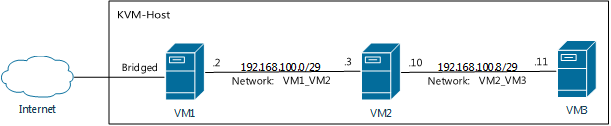
\includegraphics[width=\linewidth]{appendix/kvm/network}
	\caption{Netzwerkarchitektur virtuelle Umgebung}
	\label{fig:network}
\end{figure}

Zur Realisierung dieser Struktur werden wir zwei virtuelle Netzwerke und die entsprechende Netzwerkkarten auf den virtuellen Maschinen erstellt.

\paragraph{Netzwerk VM1\_VM2} \hfill \\
Unter der Voraussetzung, dass die Datei \lstinline|VM1_VM2.xml| im aktuellen Ordner liegt (siehe Listing\nobreak\ \ref{list:VM1_VM2.xml}), lässt sich das Netzwerk mit dem Kommando \lstinline|virsh create VM1_VM2.xml| anlegen. Libvirt generiert automatisch die entsprechende \lstinline|UUID| und eine Interface MAC-Adresse.

Mit \lstinline|virsh net-autostart VM1_VM2| stellen wir die automatische Aktivierung beim Booten sicher.

\lstinputlisting[label=list:VM1_VM2.xml,caption=\lstinline|VM1\_VM2.xml|, language=xml]{appendix/kvm/libvirt/VM1_VM2.xml}

\paragraph{Netzwerk VM2\_VM3} \hfill \\
Äquivalent dem Netzwerk VM1\_VM2 wird das Netzwerk VM2\_VM3 mit dem Kommando \lstinline[breaklines=false]|virsh create VM2_VM3.xml| erstellt. Wichtig ist hierbei, dass der \lstinline|bridge|-\lstinline|name| auf dem Hostsystem eindeutig sein muss; daher wird er hier auf \lstinline|virbr2| hochgezählt.

Mit \lstinline|virsh net-autostart VM2_VM3| stellen wir die automatische Aktivierung beim Booten sicher.

\lstinputlisting[label=list:VM2_VM3.xml,caption=\lstinline|VM2\_VM3.xml|, language=xml]{appendix/kvm/libvirt/VM2_VM3.xml}

\paragraph{Bridging Network} \hfill \\
Damit wir die VM1 von extern erreichbar machen könnten, müssten wir eine Bridge erstellen, welche auch das entsprechende physische Interface umfasst. Leider ist dies auf einer Fedora Workstation nicht ohne weiteres möglich, da der \lstinline|NetworkManager|, welcher das Netzwerk verwaltet, diese Möglichkeit nicht bietet\footnote[42]{Wie das Bridging unter Fedora konfiguriert werden kann, ist unter folgender URL ersichtlich. Wie erwähnt ist dafür aber ein deaktivieren des \lstinline|NetworkManagers| nötig.

 \url{https://docs.fedoraproject.org/en-US/Fedora/13/html/Virtualization_Guide/sect-Virtualization-Network_Configuration-Bridged_networking_with_libvirt.html}}.

Aus diesem Grund beschränken wir uns, wie im Praktikum mit den Assistenten besprochen, auf die einrichtung eines über NAT verbundenes Netzwerk. Damit ist aber von ausserhalb des Hosts kein Zugriff möglich.

Das standardmässige \lstinline|default|-Netzwerk von Libvirt ist für diesen Zweck gut geeignet. 

\lstinputlisting[
		label=list:net_default.xml,
		caption=\lstinline|/etc/libvirt/qemu/networks/default.xml|, language=xml
	]{appendix/kvm/libvirt/net_default.xml}

\subsubsection{Anlegen der Netzwerk-Interfaces mit Libvirt}

\paragraph{Interfaces VM1} \hfill \\
Um die VM1 an die beiden Netzwerke \lstinline|default| und \lstinline|VM1_VM2| anzuschliessen, muss je ein Netzwerk-Interface angelegt werden. Dies machen wir, indem wir die VM-Konfiguration mit dem Kommando \lstinline[breaklines=no]|virsh edit VM1| die beiden \lstinline|interface|-Abschnitte einfügen:

\lstinputlisting[
		label=list:vmnet_VM1.xml,
		caption=\lstinline|virsh edit VM1|: Hinzufügen Interfaces,
		language=xml
	]{appendix/kvm/libvirt/vmnet_VM1.xml}

Die obenstehenden MAC-Adressen sind generiert, und können zur automatischen Erstellung durch Libvirt auch weggelassen werden.

Wir haben uns hier für Netzwerkkarten vom Typ \lstinline|virtio| entschieden; es wäre auch möglich, andere Netzwerkkarten zu emulieren, z.B. Realtek \lstinline|rtl8139| oder Intel \lstinline|e1000|. \lstinline|virtio| ist allerdings auf einen schnellen virtuellen Betrieb optimiert, und wird von CirrOS/Linux gut unterstützt.

\paragraph{Interfaces VM2} \hfill \\
Bei der VM2 führen wir die gleichen Schritte wie für die VM1 durch, allerdings mit einer entsprechend angepasster Konfiguration:

\lstinputlisting[
		label=list:vmnet_VM2.xml,
		caption=\lstinline|virsh edit VM2|: Hinzufügen Interfaces,
		language=xml
	]{appendix/kvm/libvirt/vmnet_VM2.xml}

\paragraph{Interfaces VM3} \hfill \\
Bei der VM3 führen wir die gleichen Schritte wie für die VM1 und VM2 durch, allerdings mit einer entsprechend angepasster Konfiguration:

\lstinputlisting[
		label=list:vmnet_VM3.xml,
		caption=\lstinline|virsh edit VM3|: Hinzufügen Interfaces,
		language=xml
	]{appendix/kvm/libvirt/vmnet_VM3.xml}

\subsubsection{Netzwerkkonfiguration innerhalb der VMs}

Damit die CirrOS-VMs auf die Netzwerke zugreifen können, müssen die Interfaces noch konfiguriert werden. Dafür müssen wir die VMs zuerst starten (mehr Details dazu im Abschnitt\nolinebreak\  \ref{sec:starten-stoppen-etc-einer-virtuellen-maschine}):
\begin{lstlisting}
virsh start VM1
virsh start VM2
virsh start VM3
\end{lstlisting}

\paragraph{Konfiguration VM1} \hfill \\
Wir können uns mit \lstinline|virsh console VM1| auf die VM1 verbinden. Sobald der Bootvorgang abgeschlossen ist, loggen wir uns mit dem Standardlogin ''cirros'' und Passwort ''cubswin:)'' ein, und editieren die Netzwerk-Konfiguration mit \lstinline[breaklines=no]|sudo vi /etc/network/interfaces|

Nun müssen folgende Zeilen in der Datei existieren bzw. hinzugefügt werden:

\lstinputlisting[
		label=list:vmnet_VM1.iface,
		caption=VM1 \lstinline|/etc/network/interfaces|
	]{appendix/kvm/libvirt/vmnet_VM1.iface}

Nach dem anpassen der Konfiguration fahren wir die VM mit \lstinline|sudo poweroff| wieder herunter.

\paragraph{Konfiguration VM2} \hfill \\
Bei der VM2 gehen wir gleich vor wie bei VM1, mit dem unterschied der nachfolgenden Konfiguration von \lstinline|/etc/network/interfaces|:

\lstinputlisting[
label=list:vmnet_VM2.iface,
caption=VM2 \lstinline|/etc/network/interfaces|
]{appendix/kvm/libvirt/vmnet_VM2.iface}

Nach dem anpassen der Konfiguration fahren wir die VM mit \lstinline|sudo poweroff| wieder herunter.

\paragraph{Konfiguration VM3} \hfill \\
Bei der VM2 gehen wir gleich vor wie bei VM1 und VM2, mit dem unterschied der nachfolgenden Konfiguration von \lstinline|/etc/network/interfaces|:

\lstinputlisting[
label=list:vmnet_VM3.iface,
caption=VM3 \lstinline|/etc/network/interfaces|
]{appendix/kvm/libvirt/vmnet_VM3.iface}

Nach dem anpassen der Konfiguration fahren wir die VM mit \lstinline|sudo poweroff| wieder herunter.


\subsection{Starten, stoppen etc. einer virtuellen Maschine}\label{sec:starten-stoppen-etc-einer-virtuellen-maschine}\label{sec:starten-stoppen-etc-einer-virtuellen-maschine}

Nachdem wir nun erfolgreich die virtuelle Umgebung eingerichtet haben, wird in den folgenden Abschnitten erläutert, wie virtuelle Maschinen gestartet, heruntergefahren und auf die virtuelle Konsole zugegriffen werden kann.

\subsubsection{Mit Libvirt}
Libvirt stellt für das verwalten von virtuellen Maschinen bequeme Kommandos mit dem \lstinline|virsh|-Tool bereit, wie in den nachfolgenden Beispielen mit \lstinline|VM1| aufgezeigt.

\begin{lstlisting}[language=bash]
# VM1 starten
virsh start VM1

# Konsole der VM1 oeffnen
virsh console VM1

# ACPI-Signal zum herunterfahren an VM1 senden
virsh shutdown VM1
\end{lstlisting}


\subsubsection{Ohne Libvirt}\label{sec:ohne-libvirt}

Ohne die steuernde Funktion von Libvirt (bzw. genauer gesagt, der Steuerung von \lstinline|libvirtd| mittels \lstinline|virsh|), wird das starten und laufen lassen von virtuellen Maschinen deutlich komplizierter.

Da ohne Libvirt die Konfiguration auch nicht mit XML-Dateien erfolgt, muss die gesamte Konfiguration als Parameter zum QEMU-Aufruf mitgegeben werden. Für die VM1, wie sie bei dieser Aufgabe erstellt wird, führt \lstinline|libvirtd| folgendes Kommando durch:

\begin{lstlisting}[language=bash]
/usr/bin/qemu-system-x86_64 -machine accel=kvm -name VM1 -S -machine pc-i440fx-2.4,accel=kvm,usb=off -cpu SandyBridge,+osxsave,+pcid,+pdcm,+xtpr,+tm2,+est,+smx,+vmx,+ds_cpl,+monitor,+dtes64,+pbe,+tm,+ht,+ss,+acpi,+ds,+vme -m 512 -realtime mlock=off -smp 1,sockets=1,cores=1,threads=1 -uuid 1637255f-352a-474d-9964-071af0e8e15e -nographic -no-user-config -nodefaults -chardev socket,id=charmonitor,path=/var/lib/libvirt/qemu/VM1.monitor,server,nowait -mon chardev=charmonitor,id=monitor,mode=control -rtc base=utc,driftfix=slew -global kvm-pit.lost_tick_policy=discard -no-hpet -no-shutdown -global PIIX4_PM.disable_s3=1 -global PIIX4_PM.disable_s4=1 -boot strict=on -device ich9-usb-ehci1,id=usb,bus=pci.0,addr=0x4.0x7 -device ich9-usb-uhci1,masterbus=usb.0,firstport=0,bus=pci.0,multifunction=on,addr=0x4 -device ich9-usb-uhci2,masterbus=usb.0,firstport=2,bus=pci.0,addr=0x4.0x1 -device ich9-usb-uhci3,masterbus=usb.0,firstport=4,bus=pci.0,addr=0x4.0x2 -drive file=/var/lib/libvirt/images/vm1.qcow2,if=none,id=drive-virtio-disk0,format=qcow2 -device virtio-blk-pci,scsi=off,bus=pci.0,addr=0x3,drive=drive-virtio-disk0,id=virtio-disk0,bootindex=1 -netdev tap,fd=23,id=hostnet0,vhost=on,vhostfd=24 -device virtio-net-pci,netdev=hostnet0,id=net0,mac=52:54:00:9d:f7:54,bus=pci.0,addr=0x2 -netdev tap,fd=25,id=hostnet1,vhost=on,vhostfd=26 -device virtio-net-pci,netdev=hostnet1,id=net1,mac=52:54:00:09:17:8a,bus=pci.0,addr=0x6 -chardev pty,id=charserial0 -device isa-serial,chardev=charserial0,id=serial0 -device virtio-balloon-pci,id=balloon0,bus=pci.0,addr=0x5 -msg timestamp=on
\end{lstlisting}

Essenziell im obenstehendem Aufruf ist insbesondere \lstinline|-machine accel=kvm|; damit erfolgt die Aktivieren der KVM-Schnittstelle (falls dies weggelassen wird, führt QEMU eine Vollvirtualisierung durch).

Selbstverständlich läuft die VM nur solange, wie auch \lstinline|qemu| ausgeführt wird. Für einen produktiven Einsatz müsste dieser Aufruf also von einem Daemon ausgeführt werden.

Deshalb wird in der Praxis üblicherweise  \lstinline|libvirtd| eingesetzt.

\section{Docker}
\subsection{Grundlegendes}
Docker ist im Gegensatz zu KVM keine Lösung für virtuelle Maschinen (und damit unabhängige Betriebssysteme mit eigenem CPU-Scheduling etc.) sondern basiert auf Linux Container (LXC). Ein LXC ist eine vom Kernel bereitgestellte virtuelle Umgebung zur isolierten Ausführung von Prozessen. \\

Docker ermöglicht neben der Steuerung von isolierten Applikationsausführung in LXC die Konfiguration von Netzwerkeinstellungen bzw. Portfreigabe ein komplett isoliertes Dateisystem pro Applikation (sogenannte Images). Damit ist es möglich, Systemunabhängig immer die gleiche Plattform zur Ausführung zu paketieren und weiter zu verteilen. Von Docker erstellte Images werden üblicherweise mit einem Dateisystem erstellt, welches Snapshots erlaubt (z.B. AUFS oder BTRFS). Die Filesysteme sind ebenfalls ''stappelbar'', so dass nur die Änderungen gespeichert werden müssen. \\

Zur Erstellung von eigenen Images, auf deren Basis eine Applikation ausgeführt wird, können mit einem \lstinline[]|Dockerfile| komplette ''Bauanleitungen'' erstellt werden. Im \lstinline[]|Dockerfile| sind die Eigenschaften des neuen Container und Images sowie darauf auszuführende Kommandos zur Bereitstellung der Umgebung hinterlegt. \\

So gebaute Images (oft in diesem Zusammenhang auch einfach als Container bezeichnet) können über eine Online-Plattform verteilt werden. Die Firma Docker Inc. stellt zu diesem Zweck die öffentliche Plattform \emph{DockerHub} unter \url{https://hub.docker.com/} zur Verfügung. \\

Ein öffentliches Image kann wie folgt adressiert werden \lstinline[]|<author name>/<image name>:<tag>|. Der Teil vor dem Doppelpunkt wird Repository genannt. Ein Repository kann in mehreren Versionen vorliegen. Diese Versionen werden anhand eines Tags unterschieden, welcher hinter Doppelpunkt steht. Wird kein Tag angegeben, wird automatisch das aktuellste (latest) Image verwendet. \\

Daten die im Docker Image erzeugt werden, verschwinden nach dem Beenden des Containers. Um Daten Persistent zu speichern muss ein lokales Verzeichnis mit einem Verzeichnis des Hostsystems gemappt werden. Dies geschieht mit dem Parameter \lstinline[]|-v ./host_folder:/var/container_folder| \\

Beim Bauen eines Containers wird üblicherweise auf die Basis eines bestehenden Containers auf der DockerHub-Plattform zurückgegriffen. So gibt es dort zum Beispiel Images, welche die Dateisystemstruktur und Bibliotheken eines minimalen Ubuntu-Systems oder sogar einer Umgebung für  wie Ruby on Rails zur Verfügung stellen. \\

Docker funktionierte anfänglich nur für 64 Bit Linux Distributionen. Später kam der Support für MacOSX hinzu und seit neustem läuft Docker auch unter Windwos, wobei Hyper-V für die Virtualisierung der Docker Engine und Linux spezifischen Kernel Features verwendet wird.

\subsubsection{Terminologie}
\begin{description}
	\item[Image] Eine portable Abbildung eines Containers.
	\item[Container] Lauffähiges virtuelles System. Instanz eines Images.
	\item[Dockerfile] Ist eine Textdatei, in welcher der Aufbau eines Docker Images beschrieben ist.
	\item[Docker Hub] ein Online-Dienst, der eine Registry für Docker-Images und Repositorys beinhaltet
	\item[Libcontainer] Libcontainer ist eine Schnittstelle für die Grundfunktionalitäten von Docker. Es ersetzt die LXC Schnittstelle die anfänglich verwendet wurde. 
	\item[libswarm]eine Schnittstelle um Docker-Container zu steuern.
	\item[libchan] eine Schnittstelle zu Dockers Netzwerkfunktionen.
\end{description}

\subsubsection{Ordner}
\begin{description}
	\item[/var/lib/docker/containers/] Hier liegen alle Container
	\item[/var/lib/docker/devicemapper/devicemapper/data] Hier liegen alle Images
\end{description}

\subsubsection{Docker Compose}
Docker Compose ist ein ergänzendes Programm zu Docker, welches die Orchestrierung von mehreren Docker-Containern erlaubt. Docker Compose vereinfacht also die Verwaltung und das Linking von mehreren Docker Container. Der Aufbau/Start der Container wird mittels dem Kommando \lstinline|docker-compose| gesteuert; dies liest die \lstinline|docker-compose.yml|-Datei ein, in welcher weitergehende Anweisungen für die Konfiguration der Container definiert sind.

\subsubsection{Docker Swarm}
Docker Swarm erlaubt das Verknüpfen mehrerer Docker Hosts zu einem Cluster. Ein Swarm besteht immer aus einem Master, einem Discovery Service und mehreren Nodes. Mit Hilfe von Docker Machine können beliebig viele Nodes erstellt werden. Ein Container der in einem Swarm deployed wird, wird gemäss einem bestimmten Strategie (spread, binpack, random) auf den verfügbaren Nodes verteilt. Mit dem Befehl \lstinline[]|docker service scale <service_id>=<number_of_tasks>| kann ein Service leicht skaliert werden.

\begin{figure}[h]
	\centering
	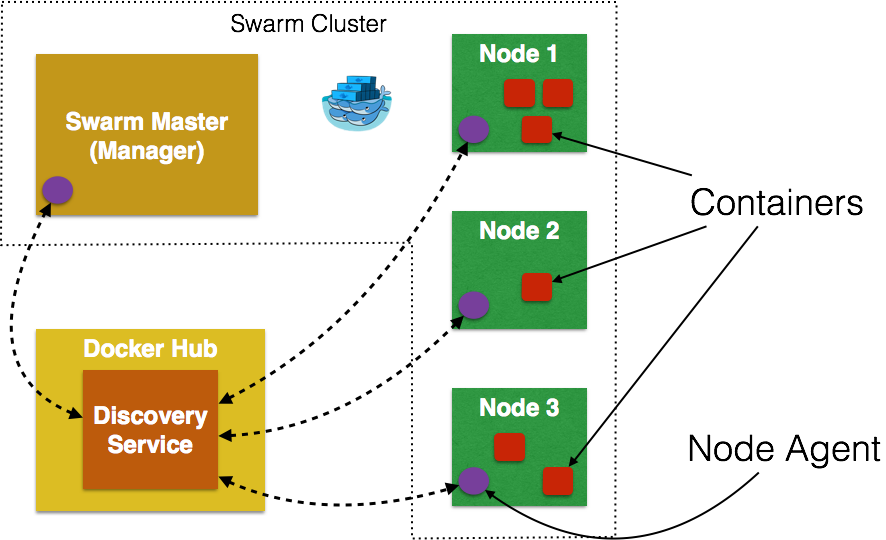
\includegraphics[width=0.5\linewidth]{appendix/docker/docker-swarm-cluster}
	\caption{Docker Swarm Key Components}
	\label{fig:docker-swarm-cluster}
\end{figure}

\subsubsection{Docker Machine}
Docker Machine ist ein Tool um die Docker Engine auf virtuellen Hosts zu installieren und verwalten. Es ist zurzeit die einzige Möglichkeit, um Docker auf Mac oder Windows laufen zu lassen. Ebenfalls lassen sich Swarm Cluster damit erstellen. Unter Fedora wird Docker Machine wie folgt installiert:
\begin{lstlisting}[language=bash]
curl -L https://github.com/docker/machine/releases/download/v0.8.2/docker-machine-`uname -s`-`uname -m` >/usr/local/bin/docker-machine && \ chmod +x /usr/local/bin/docker-machine
\end{lstlisting}

\subsection{Docker IO}
Folgend einige wichtige Kommandos die unter Docker oft gebraucht werden.
\begin{lstlisting}[language=bash]
# docker image suchen
docker sarch <package-name>

# docker image starten
docker run <package-name> <app to execute>

# docker image herunterladen
docker pull <package-name>

# Image veroeffentlichen
docker push <image name>

# Liste alle lokal vorliegenden Images
docker images

# Image entfernen
docker rmi <image>

# erzeuge image aus Dockerfile
docker build <repository>

# Aktuell ausgefuerten Container anzeigen
docker ps

# Docker container stopen / starten
docker (stop|start) <name>/<id>

# Container entfernen
docker rm <container>
\end{lstlisting}

\subsection{ELK Stack Setup (Elasticseach, Logstash, Kibana)}
\begin{description}
	\item[Elasticsearch] Elasticsearch ist eine mandantenfähige Suchengine für Volltextsuchen. Es verfügt über ein RESTful Webinterface.
	\item[Logstash] Mit Logstash können Events und Log Meldungen gesammelt, verarbeitet und weitergeleitet werden. Die Daten werden über diverse Input Plugins gesammelt und anschliessend innerhalb von Logstash gefiltert werden. Der resultierende Output wird dann an Elasticsearch weitergereicht.
	\item[Kibana] Kibana ist ein Open Source Plugin für die Visualisierung der Daten innerhalb von Elasticsearch. 
\end{description}

\subsubsection{Ports}
\begin{itemize}
	\item 5601 - Kibana web interface
	\item 9200 - Elasticsearch HTTP (JSON Interface)
	\item 9300 - Elasticsearch TCP transport
	\item 5000 - Logstash Lumberjack interface, receives logs from Logstash forwarders
\end{itemize}

\subsection{Vorraussetzungen}
\subsubsection{Docker Installation}
Folgende Schritte sind notwendig um Docker unter Fedora verwenden zu können.
\begin{lstlisting}[language=bash]
# add repository
sudo tee /etc/yum.repos.d/docker.repo <<-'EOF'
	[dockerrepo]
	name=Docker Repository
	baseurl=https://yum.dockerproject.org/repo/main/fedora/$releasever/
	enabled=1
	gpgcheck=1
	gpgkey=https://yum.dockerproject.org/gpg
	EOF

# install docker
sudo dnf install docker-engine

# enable service
sudo systemctl enable docker.service

# start service
sudo systemctl start docker

# check installation
sudo docker run --rm hello-world
\end{lstlisting}

\subsubsection{VirtualBox}
Damit wir eine Testumgebung für Docker Swarm aufbauen können, muss eine aktuelle Version von VirtualBox vorliegen.  Dies wird unter Fedora wie folgt installiert:
\begin{lstlisting}[language=bash]
cd /etc/yum.repos.d/ 
sudo wget http://download.virtualbox.org/virtualbox/rpm/fedora/virtualbox.repo
sudo dnf update

dnf install binutils gcc make patch libgomp glibc-headers glibc-devel kernel-headers kernel-devel dkms

KERN_DIR=/usr/src/kernels/`uname -r`
\end{lstlisting}


\subsubsection{SELinux} \hfill \\
Da wir mit einem Fedora arbeiten, muss vorgängig der SELinux Security Context für den Order in dem die Container zu liegen kommen, angepasst werden. Dazu erstellen wir einen Ordner \lstinline[]|docker-elk| und wechseln anschliessend in den übergeordneten Folder.
\begin{lstlisting}[language=bash]
mkdir docker-elk
cd ..
chcon -R system_u:object_r:admin_home_t:s0 docker-elk
\end{lstlisting}

\subsubsection{Max Map Count}
Der Max Map Count beinhaltet die maximale Anzahl an Memory Map Area's die einem Prozess zugeordnet werden können. Memory Map Areas werden bei der Verwendung von \lstinline[]|malloc| genutzt. Damit Docker genügend Areas zur Verfügung stehen, setzen wir den default von 65536 auf 262144.
\begin{lstlisting}[language=bash]
sudo sysctl -w vm.max_map_count=262144
\end{lstlisting}

\subsection{Docker Images}
In einem ersten Schritt wird innerhalb des \lstinline[]|docker-elk| Folder, für jede Komponente ein eigener Ordner angelegt.(\lstinline[]|mkdir logstash elasticsearch kibana|). Anschliessend wird für jede Komponente ein Dockerfile angelegt, welches auf ein bestehendes Docker Hub Image zurückgreift. (\lstinline[]|touch Dockerfile|). Alle Teilkomponenten setzen dabei auf die aktuellste Version 5 des Basis Containers.

\subsubsection{Docker File}
Ein Dockerfile beschreibt wie ein Docker Image erstellt werden soll. 
\begin{description}
	\item[FROM] Der wichtigste Befehl im Dockerfile ist FROM. Dieser muss ganz oben stehen und beschreibt ganz einfach, welches Image die Grundlage für das neu erzeugtes Image ist.	
	\item[RUN] Führt einen Befehl innerhalb des Containers aus
	\item[COPY] Kopiert ein File in das Filesystem des Containers
	\item[CMD] Bietet einen Defaultcommand für einen ausgeführten Container. Es gibt nur einen CMD Befehl pro Docker Image.
	\item[EXPOSE] Veröffentlicht eine Port nach aussen
	\item[ENV] Setzt eine Umgebungsvariable
\end{description}

\subsubsection{Elasticsearch}
\begin{lstlisting}[caption=Elasticsearch Dockerfile, language=bash]
FROM elasticsearch:5

ENV ES_JAVA_OPTS="-Des.path.conf=/etc/elasticsearch"

CMD ["-E", "network.host=0.0.0.0", "-E", "discovery.zen.minimum_master_nodes=1"]
\end{lstlisting}

\subsubsection{Logstash} 
\begin{lstlisting}[caption=Logstash Dockerfile, language=bash]
FROM logstash:5
\end{lstlisting}

Für die konfiguraiton von Logstash ist noch ein zusätzliches Config File nötig. Dieses definiert auf einfache Art und Weise auf welchem Port die Daten empfangen und auf welchem Port die Daten an Elasticsearch weitergereicht werden.
\begin{lstlisting}
input {
	tcp {
		port => 5000
	}
}

output {
	elasticsearch {
		hosts => "elasticsearch:9200"
	}
}
\end{lstlisting}

\subsubsection{Kibana} 
\begin{lstlisting}[caption=Kibana Dockerfile, language=bash]
FROM kibana:5

# precondition to open tcp connection on given port
RUN apt-get update && apt-get install -y netcat

# copy script from host to kibana container
COPY startup.sh /tmp/startup.sh

# mark as executable
RUN chmod +x /tmp/startup.sh 

# execute
CMD ["/tmp/startup.sh"] 
\end{lstlisting}

Da Kibana die Daten aus Elasticsearch visualisert, muss sichergestellt werden, dass der Elasticsearch Container bereits läuft, bevor Kibana gestartet wird. Dies erledigen wir mit einem einfach Polling Script. Für das Polling wird \lstinline[]|nc| (Netcat) benötigt, welches im Dockerfile via \lstinline[]|apt-get install ncat| installiert wird. 
\begin{lstlisting}[caption=Kibana Pooling Script, language=bash]
#!/bin/bash

# Wait for the Elasticsearch container to be ready before starting Kibana.
echo "Waiting for Elasticsearch"
while true; do
	nc -q 1 elasticsearch 9200 2>/dev/null && break
	
	# sleep for a second to save cpu
	sleep 1
done

echo "Starting Kibana"
exec kibana
\end{lstlisting}

Auch für Kibana gibt es eine Config. In dieser definieren wird die grundlegenden Einstellungen.	
\begin{lstlisting}[caption=kibana.yml, language=bash]
# Port by which Kibana is served
server.port: 5601

# IP address of the back end server. (localhost)
server.host: "0.0.0.0"

# Elasticsearch URL
elasticsearch.url: "http://elasticsearch:9200"
\end{lstlisting}


\subsection{Docker Compose File}
Im Composer File werden die vorgehenden Dockerfiles orchestriert.
\begin{description}
	\item[build] Order in welchem das Docker File liegt
	\item[ports] Ports welche an das Hostsystem weitergeleitet werden sollen
	\item[networks (local)] \hfill \\ In welchem Netzwerk arbeitet ein Container. Weitere Informationen im Absatz \ref{sec:docker_networkconf}
	\item[networks (global)] Definition der benötigten Bridge Netzwerke
\end{description}
\begin{lstlisting}[caption=docker-compose.yml Compose File, language=bash]
version: '2'

services:
	elasticsearch:
		build: elasticsearch
		environment:
			ES_JAVA_OPTS: "-Xms1g -Xmx1g"
		networks:
			KIBANA_ELASTIC:
				ipv4_address: 192.168.120.2
			LOGSTASH_ELASTIC:
				ipv4_address: 192.168.120.10
	logstash:
		build: logstash/
		command: -f /etc/logstash/conf.d/
		volumes:
			- ./logstash/config:/etc/logstash/conf.d
		ports:
			- "${IFADDR_MGMT}:5000:5000"
		networks:
			LOGSTASH_ELASTIC:
				ipv4_address: 192.168.120.11
	kibana:
		build: kibana/
		volumes:
			- ./kibana/config/:/opt/kibana/config/
		ports:
			- "${IFADDR_IT}:5601:5601"
		networks:
			KIBANA_ELASTIC:
				ipv4_address: 192.168.120.3

networks:
	KIBANA_ELASTIC:
		driver: bridge
		ipam:
			config:
				- subnet: 192.168.120.0/29
	LOGSTASH_ELASTIC:
		driver: bridge
		ipam: 
			config:
				- subnet: 192.168.120.8/29
\end{lstlisting}

\subsubsection{Test}
Wenn alle vorgängigen Files wie beschrieben erstellt wurden, kann der ELK Stack gestartet werden. Das Webinterface ist fortan unter \url{http://localhost:5601/} verfügbar. Das Default Login für Kibana lautet \lstinline[]|'kibana'| mit dem Passwort \lstinline[]|'changeme'|
\begin{lstlisting}[language=bash]
IFADDR_IT=<eth0 ipv4 addr> IFADDR_MGMT=<eth1 ipv4 addr> docker-compose up
\end{lstlisting}

Um Kibana mit Dummy Daten zu füttern, kann folgender Befehl ausgeführt werden: \lstinline[]|sudo nc localhost 5000 < /var/log/<any_logfile>.log|

\subsection{Netzwerkkonfiguration}
Docker erstellt standardmässig ein Netzwerk Interface (\lstinline[]|docker0|) im Adressbreich 172.17.x.x/16. Wurde kein spezifisches Netzwerk angegeben(\lstinline[]|docker run --network <net name>|), sind alle Container standardmässig an dieses Interface gebunden. Ebenfalls werden drei Docker interne Netzwerke angelegt.
\begin{lstlisting}[language=bash]
# sudo docker network ls

NETWORK ID          NAME                DRIVER
d8159c421bee        bridge              bridge              
e98ecb6fefeb        none                null                
427ea6518c34        host                host    
\end{lstlisting}

\subsubsection{Übersicht}
\label{sec:docker_networkconf}
Um die Vorgaben an die Netzwerkkonfiguration zu erfüllen, haben wir uns für eine statische Konfiguration entschieden. Dafür werden im Docker Compose zwei Bridge Interfaces eingerichtet. Das Erste verbindet Kibana mit Elasticsearch in dem Subnetz 192.168.120.0/29 und das Zweite verbindet Elasticsearch mit Logstash in dem Subnetz 192.168.120.8/29. Der Port 5000 wird in das Netzwerk Management des Host Systems gemappt. Die externe Adresse kann über die Umgebungsvariable \lstinline[]|IFADDR_IT| gesetzt werden. Der Port 5601 für das Kibana Webinterface soll nur aus dem IT Netz erreichbar sein. Die externe Management Adresse kann über die Umgebungsvariable \lstinline[]|IFADDR_MGMT| gesetzt werden.
\begin{figure}[h]
\centering
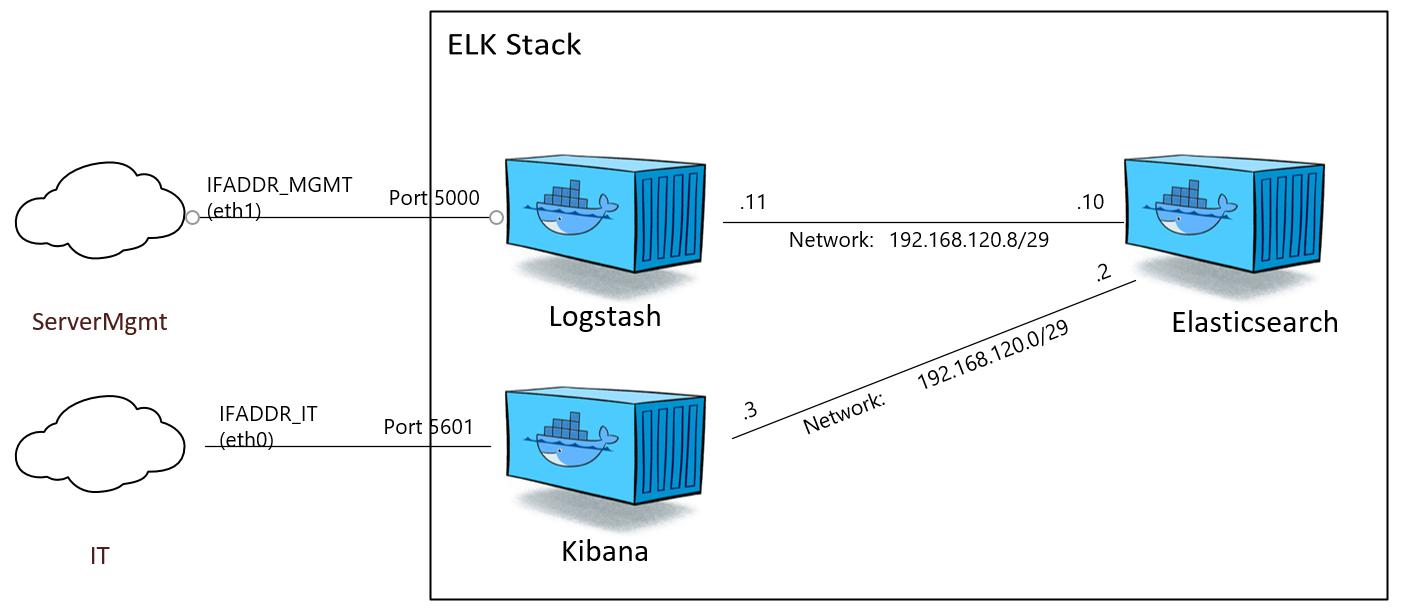
\includegraphics[width=0.7\linewidth]{images/docker_network_conf}
\caption{Übersicht Netzwerkkonfiguration}
\label{fig:dockernetworkconf}
\end{figure}
\newpage


\subsubsection{Tests}
Um die Netzwerkkonnektivität zu überprüften schalten wir uns bei laufendem ELK Stack auf die einzelnen Container drauf:
\begin{lstlisting}[language=bash]
sudo docker exec -ti <container> /bin/bash

#  list ip addr
ip addr 

# check connectivity
ping 192.168.120.2
\end{lstlisting}

\subsection{Docker Swarm}
Docker Swarm dient der Orchestrierung mehrere Docker Machines zu einem übergreifenden Cluster.

\subsubsection{Umgebungsvariablen}
Bei der Erstellung der Swarm Nodes werden automatisch TLS Zertifikate installiert, damit diese auch gefunden werden muss unter \lstinline[]|/etc/sysconfig/docker| folgendes IF Statement hinzugefügt werden. 
\begin{lstlisting}[caption=/etc/sysconfig/docker, language=bash]
if [ -z "${DOCKER_CERT_PATH}" ]; then
	DOCKER_CERT_PATH=/etc/docker
fi
\end{lstlisting}

\subsection{Docker Swarm Cluster Erstellen}
Docker Swarm bietet mehrere Discovery Backends. Ein Discovery Service verwaltet eine Liste von IPs innerhalb des Docker Swarm Cluster. Da die Container in diesem Lab nicht in einer produktiven Umgebung zum Einsatz kommen, verwenden wir als Discovery Service einen einfachen Token der von Docker Hub generiert wird. Ebenefalls erstellen wir einen Swarm Manager, der alle Node im Swarm Cluster orchestriert.

\begin{lstlisting}[language=bash]
docker-machine create -d virtualbox local

eval "$(docker-machine env local)"

# Generate a discovery token using the Docker Swarm image.
docker run swarm create

# Wichtig: hier muss der Token am Ende des Outputs sicheraufbewahrt werden: 
8c39e2080809189e0169ef1f468463d3

# create swarm manager
docker-machine create -d virtualbox --swarm --swarm-master --swarm-discovery token://8c39e2080809189e0169ef1f468463d3 swarm-master

# create nodes
docker-machine create -d virtualbox --swarm --swarm-discovery token://8c39e2080809189e0169ef1f468463d3 node01

docker-machine create -d virtualbox --swarm --swarm-discovery token://8c39e2080809189e0169ef1f468463d3 node01
\end{lstlisting}

\section{Vergleich der Technologien}

Auf der Abbildung \ref{fig:dockervirtualization} ist übersichtlich dargestellt, wie die unterschiedlichen Stacks mit virtual Machines (KVM) und Containers (Docker) aufgebaut sind. In Tabelle \ref{tabu:kvm-docker} auf der nächsten Seite werden die unterschiedlichen Ansätze der beiden Technologien gegenübergestellt.

\begin{figure}[h]
\centering
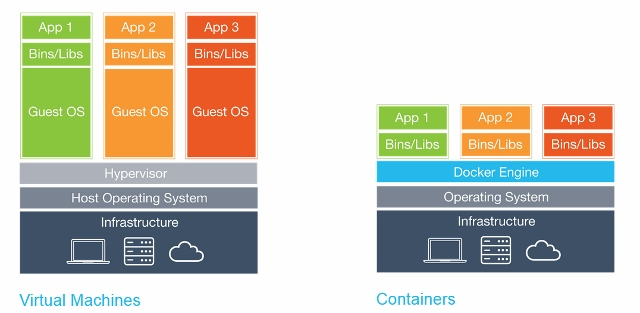
\includegraphics[width=0.7\linewidth]{images/docker_virtualization}
\caption{Docker vs KVM Virtualization}
\label{fig:dockervirtualization}
\end{figure}

\pagebreak
\begin{table}[H]
	\centering
	\begin{tabu} to \linewidth {r | X X}
		\toprule
		\textbf{Vergleich} & \textbf{KVM/QEMU} & \textbf{Docker} \\
		\midrule
		Isolationsebene & Komplettes Betriebssystem & Applikation mit Libraries \\ \hline
		Persistenz & Dateisystem ist persistent (und somit eher teuer). & Dateisystem flüchtig; Daten müssen in Datencontainer  oder extern ausgelagert werden \\ \hline
		Lebenszyklus & Hoher Installationsaufwand, lange Betriebszeit (meist 3-15 Jahre) & Kleiner Installationsaufwand, kurze Lebenszeit (oft wenige Monate) \\ \hline
		Applikationsdichte & je nach dem 1 - 1000 pro VM & Üblicherweise 1 pro Container \\ \hline
		Systemupdate & Updates können üblicherweise einmal pro VM installiert werden. & Updates müssen auf allen Containern ausgerollt werden \\ \hline
		Speicherbedarf & Vollständiges Betriebssystem mit allen Abhängigkeiten; kann dafür für mehrere Applikationen verwendet werden & Üblicherweise Image mit den meisten Betriebssystembibliotheken; kann von mehren Docker Containern via Overlay genutzt werden \\ \hline
		Memorybedarf & Systemaufgaben; Libraries sind oft geshared, also einmal im Memory & Keine gesharte libraries; alles mehrfach im Memory \\ \hline
		CPU & Eigenes Scheduling; dadurch viel System-Overhead & Scheduling etc. wird vom Host durchgeführt, relativ effizient. \\ \hline
		Skalierbarkeit & Aufwändig; nur bis zu einem gewissen Grad ausbaubar & Einfach: neue Instanzen der Docker-Container hinzufügen. \\ \hline
		Reproduzierbarkeit\textsuperscript{43} & Eher aufwändig/teuer (VM-Klon), nicht nur eine Applikation, braucht VM-Umgebung & Sehr einfach: Container sind weitgehend atomar und laufen (beinahe) überall\\ \hline
		Orchestrierung & Eher schwierig; z.B. mit Puppet, Chef, Salt, Ansible möglich & Einfach: direkt von Docker mit Compose \& Swarm unterstützt \\ \hline
		Migrationsaufwand & Bestehende Applikationen laufen ohne Probleme & Die meisten Applikationen müssen angepasst werden (z.B. betreffend Datenablage) \\ \hline
		Systemsupport & Grundsätzlich alle Systeme & z:Z. nur UNIXartige Applikationen \\ \hline
		Eignung & Klassische, eng verzahnte Applikationsumgebungen mit vielen abhängigen Prozessen & Isolierte/Atomare Applikationen mit wenigen und unabhängigen Prozessen \\ \hline
		Typisches Beispiel & Klassischer LAMP-Stack & ELK-Stack, Node.js Webapp \\
		\bottomrule
	\end{tabu}
	\caption{Gegenüberstellung KVM/QEMU und Docker}
	\label{tabu:kvm-docker}
\end{table}
\footnotetext[43]{Damit ist gemeint, wie kompliziert das Aufsetzen einer genau gleichartigen Umgebung z.B. für Entwicklungs- oder Stagingsysteme ist.}
\pagebreak


\subsection{Docker}
\paragraph{Vorteile}
\begin{itemize}
	\item Man kann auf den Ballast eines kompletten Betriebssystems verzichten, wenn man nur eine Applikation isoliert ausführen möchte.
	\item Äusserts sparsamer Umgang mit Ressourcen und eine kurze Startzeit	sobald die Images einmal gepullt wurden.
	\item Sehr einfach einen Docker Container zu installieren
	\item Austausch von Images fällt durch den Gebrauch von öffentlichen Registries leicht. (Docker Hub)
	\item Container sind portalbel und bietet auf jedem Host eine einheitliche Umgebung
	\item Mittels Docker Swarm und Docker Machine skalierbar
\end{itemize}
\paragraph{Nachteile}
\begin{itemize}
	\item Da die Container auf den Linux Kernel zugreifen, ist es nicht möglich Windows Anwendungen in einem Docker Container auszuführen.
	\item Der Docker Daemon läuft mit Root Rechten. Eine Sicherheitslücke in einem einzelnen Container kann das gesamte Host System kompromittieren
\end{itemize}

\subsection{KVM} %TODO
\paragraph{Vorteile}
\begin{itemize}
	\item Ein Vorteil von KVM ist, dass die Gastsysteme fast mit nativer Geschwindigkeit laufen, d.h. das Gastsystem reagiert nahezu so schnell wie ein natives System. 
\end{itemize}
\paragraph{Nachteile}
\begin{itemize}
	\item Hoher Bedarf an Festplatten und Arbeitsspeicher und langwieriger Ladevorgang beim Starten der virtuellen Maschienen
\end{itemize}

\appendix

\section{Konfigurationen}
\label{appendix:configurations}

\subsection{BR1-R1}
\subsubsection{Running Configuration}
\lstinputlisting{appendix/config/br1-r1/br1-r1-config.txt}

\subsubsection{IP Interfaces}
\lstinputlisting{appendix/config/br1-r1/br1-r1-interface.txt}

\subsubsection{Interface Status}
\lstinputlisting{appendix/config/br1-r1/br1-r1-status.txt}

\subsubsection{Neighbors}
\lstinputlisting{appendix/config/br1-r1/br1-r1-neighbors.txt}

\subsection{BR2-R1}
\subsubsection{Running Configuration}
\lstinputlisting{appendix/config/br2-r1/br2-ri-config.txt}

\subsubsection{IP Interfaces}
\lstinputlisting{appendix/config/br2-r1/br2-ri-interface.txt}

\subsubsection{Interface Status}
\lstinputlisting{appendix/config/br2-r1/br2-ri-status.txt}

\subsubsection{Neighbors}
\lstinputlisting{appendix/config/br2-r1/br2-ri-neighbors.txt}

\subsection{BR2-S1}
\subsubsection{Running Configuration}
\lstinputlisting{appendix/config/br2-s1/br2-s1-config.txt}

\subsubsection{IP Interfaces}
\lstinputlisting{appendix/config/br2-s1/br2-s1-interface.txt}

\subsubsection{Interface Status}
\lstinputlisting{appendix/config/br2-s1/br2-s1-status.txt}

\subsubsection{Neighbors}
\lstinputlisting{appendix/config/br2-s1/br2-s1-neighbors.txt}

\subsection{CCNA-CCNP-FRSwitch}
\subsubsection{Running Configuration}
\lstinputlisting{appendix/config/framerelayswitch/framerelayswitch-config.txt}

\subsubsection{IP Interfaces}
\lstinputlisting{appendix/config/framerelayswitch/framerelayswitch-interface.txt}

\subsubsection{Interface Status}
\lstinputlisting{appendix/config/framerelayswitch/framerelayswitch-status.txt}

\subsubsection{Neighbors}
\lstinputlisting{appendix/config/framerelayswitch/framerelayswitch-neighbors.txt}

\subsection{HQ FrameRelay Router (HQ-FRR)}
\subsubsection{Running Configuration}
\lstinputlisting{appendix/config/hq-frr/hq-frr-config.txt}

\subsubsection{IP Interfaces}
\lstinputlisting{appendix/config/hq-frr/hq-frr-interface.txt}

\subsubsection{Interface Status}
\lstinputlisting{appendix/config/hq-frr/hq-frr-status.txt}

\subsubsection{Neighbors}
\lstinputlisting{appendix/config/hq-frr/hq-frr-neighbors.txt}

\subsection{HQ-IER1}
\subsubsection{Running Configuration}
\lstinputlisting{appendix/config/hq-ier1/hq-ier1-config.txt}

\subsubsection{IP Interfaces}
\lstinputlisting{appendix/config/hq-ier1/hq-ier1-interface.txt}

\subsubsection{Interface Status}
\lstinputlisting{appendix/config/hq-ier1/hq-ier1-status.txt}

\subsubsection{Neighbors}
\lstinputlisting{appendix/config/hq-ier1/hq-ier1-neighbors.txt}

\subsection{HQ-WER1}
\subsubsection{Running Configuration}
\lstinputlisting{appendix/config/hq-wer1/hq-wer1-config.txt}

\subsubsection{IP Interfaces}
\lstinputlisting{appendix/config/hq-wer1/hq-wer1-interface.txt}

\subsubsection{Interface Status}
\lstinputlisting{appendix/config/hq-wer1/hq-wer1-status.txt}

\subsubsection{Neighbors}
\lstinputlisting{appendix/config/hq-wer1/hq-wer1-neighbors.txt}

\subsection{HQ CS1}
\subsubsection{Running Configuration}
\lstinputlisting{appendix/config/hq-cs1/hq-cs1-config.txt}

\subsubsection{IP Interfaces}
\lstinputlisting{appendix/config/hq-cs1/hq-cs1-interface.txt}

\subsubsection{Interface Status}
\lstinputlisting{appendix/config/hq-cs1/hq-cs1-status.txt}

\subsubsection{Neighbors}
\lstinputlisting{appendix/config/hq-cs1/hq-cs1-neighbors.txt}

\subsection{HQ CS2}
\subsubsection{Running Configuration}
\lstinputlisting{appendix/config/hq-cs2/hq-cs2-config.txt}

\subsubsection{IP Interfaces}
\lstinputlisting{appendix/config/hq-cs2/hq-cs2-interface.txt}

\subsubsection{Interface Status}
\lstinputlisting{appendix/config/hq-cs2/hq-cs2-status.txt}

\subsubsection{Neighbors}
\lstinputlisting{appendix/config/hq-cs2/hq-cs2-neighbors.txt}

\subsection{HQ CS3}
\subsubsection{Running Configuration}
\lstinputlisting{appendix/config/hq-cs3/hq-cs3-config.txt}

\subsubsection{IP Interfaces}
\lstinputlisting{appendix/config/hq-cs3/hq-cs3-interface.txt}

\subsubsection{Interface Status}
\lstinputlisting{appendix/config/hq-cs3/hq-cs3-status.txt}

\subsubsection{Neighbors}
\lstinputlisting{appendix/config/hq-cs3/hq-cs3-neighbors.txt}

\subsection{HQ CS4}
\subsubsection{Running Configuration}
\lstinputlisting{appendix/config/hq-cs4/hq-cs4-config.txt}

\subsubsection{IP Interfaces}
\lstinputlisting{appendix/config/hq-cs4/hq-cs4-interface.txt}

\subsubsection{Interface Status}
\lstinputlisting{appendix/config/hq-cs4/hq-cs4-status.txt}

\subsubsection{Neighbors}
\lstinputlisting{appendix/config/hq-cs4/hq-cs4-neighbors.txt}

\subsection{HQ DS1}
\subsubsection{Running Configuration}
\lstinputlisting{appendix/config/hq-ds1/hq-ds1-config.txt}

\subsubsection{IP Interfaces}
\lstinputlisting{appendix/config/hq-ds1/hq-ds1-interface.txt}

\subsubsection{Interface Status}
\lstinputlisting{appendix/config/hq-ds1/hq-ds1-status.txt}

\subsubsection{Neighbors}
\lstinputlisting{appendix/config/hq-ds1/hq-ds1-neighbors.txt}

\subsection{HQ DS2}
\subsubsection{Running Configuration}
\lstinputlisting{appendix/config/hq-ds2/hq-ds2-config.txt}

\subsubsection{IP Interfaces}
\lstinputlisting{appendix/config/hq-ds2/hq-ds2-interface.txt}

\subsubsection{Interface Status}
\lstinputlisting{appendix/config/hq-ds2/hq-ds2-status.txt}

\subsubsection{Neighbors}
\lstinputlisting{appendix/config/hq-ds2/hq-ds2-neighbors.txt}

\subsection{HQ DS3}
\subsubsection{Running Configuration}
\lstinputlisting{appendix/config/hq-ds3/hq-ds3-config.txt}

\subsubsection{IP Interfaces}
\lstinputlisting{appendix/config/hq-ds3/hq-ds3-interface.txt}

\subsubsection{Interface Status}
\lstinputlisting{appendix/config/hq-ds3/hq-ds3-status.txt}

\subsubsection{Neighbors}
\lstinputlisting{appendix/config/hq-ds3/hq-ds3-neighbors.txt}


\section{Messungen}
\label{appendix:measures}
\subsection{Von X nach Y}
\lstinputlisting{appendix/config/br2-r1/br2-ri-config.txt}

% Code Listings
% \lstlistoflistings

% List of figures
% \listoffigures

% List of tables
% \listoftables

% Bibliography
% \bibliographystyle{plain} 
% \bibliography{literatur}

\end{document}
